\subsection{Selekcja elitarna}

Za pomocą selekcji elitarnej wybierane są osobniki, które pojawią się także w następnym pokoleniu. 

\subsubsection{Kod źródłowy}

\begin{lstlisting}[linewidth=16.0cm]
mySelection <- function (ga_object, parent)
{
   # Pobranie specjalnie wyliczonego wspolczynnika
   # o rozmiarze rownym rozmiarowi populacji
   prob <- abs(
   	cos(ga_object@fitness)/(sin(ga_object@fitness))
   )
	
   # Wektor o tym samym rozmiarze;
   # Losowo pobrane indeksy 
   # mniejsze lub rowne rozmiarowi populacji
   sel <- sample(1:ga_object@popSize, size = ga_object@popSize, 
   	prob = pmin(prob, 1, na.rm = TRUE),
   	replace = TRUE)

   # Selekcja na podstawie wektora sel
   out <- list(population = ga_object@population[sel,,drop=FALSE],
   	fitness = ga_object@fitness[sel])
   return(out)
}

\end{lstlisting}

\subsubsection{Wyniki badań}


\begin{figure}[H]
	\centering
	\hspace*{-0.8in}
	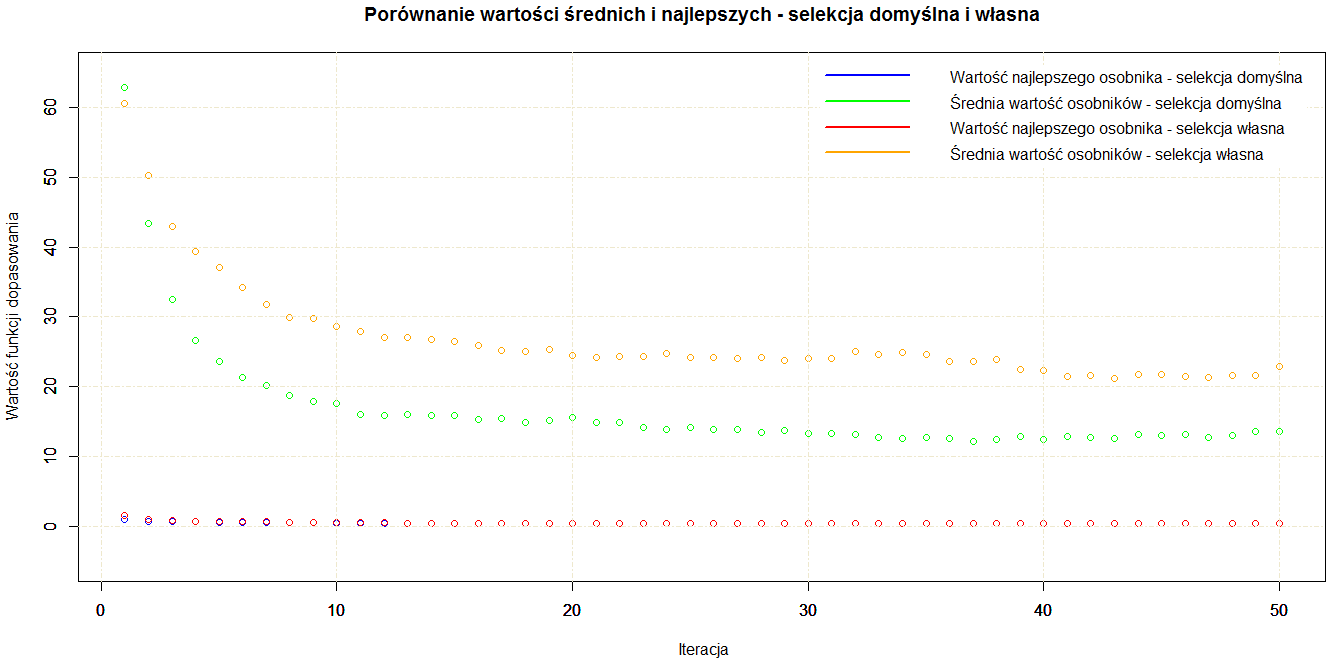
\includegraphics[scale = 0.47]{img/zad1/sel_1}
	\caption{Wykres przy 1 osobniku elitarnym}  
	\label{rys:sel_1} 
\end{figure}

\begin{figure}[H]
	\centering
	\hspace*{-0.8in}
	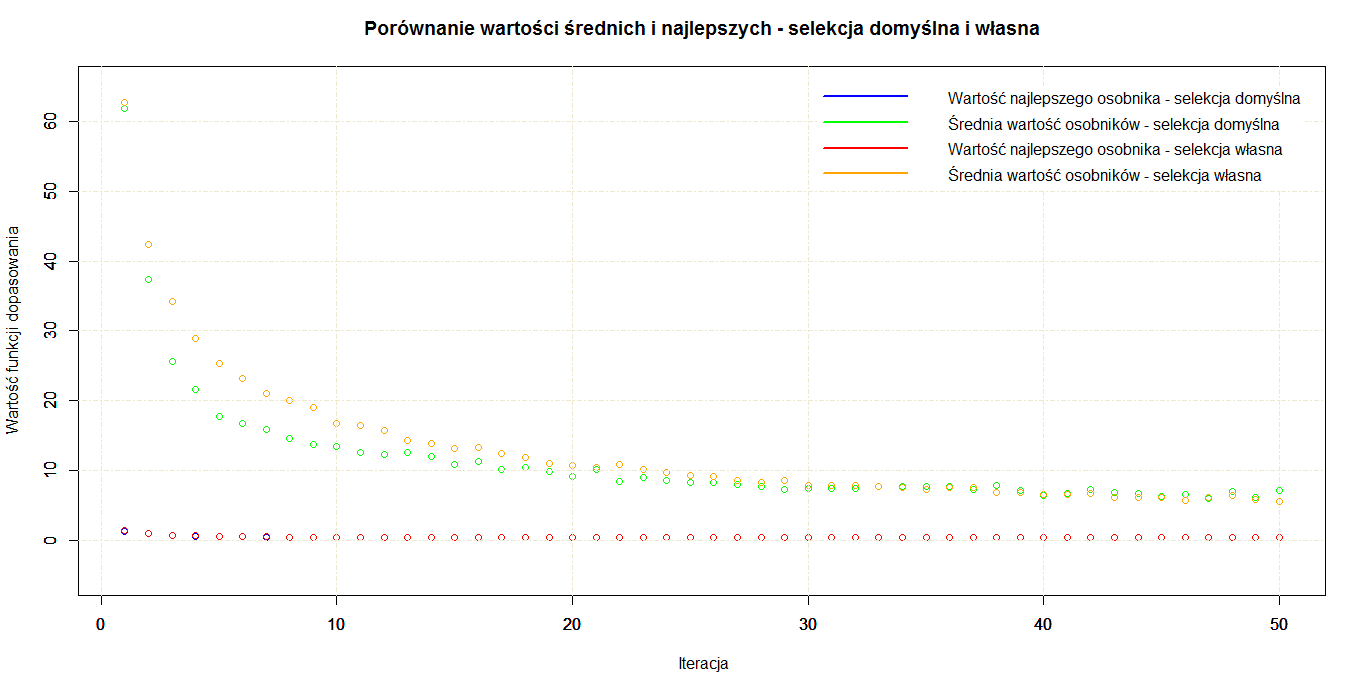
\includegraphics[scale = 0.47]{img/zad1/sel_6}
	\caption{Wykres przy 6 osobnikach elitarnych}  
	\label{rys:sel_6} 
\end{figure}

\begin{figure}[H]
	\centering
	\hspace*{-0.8in}
	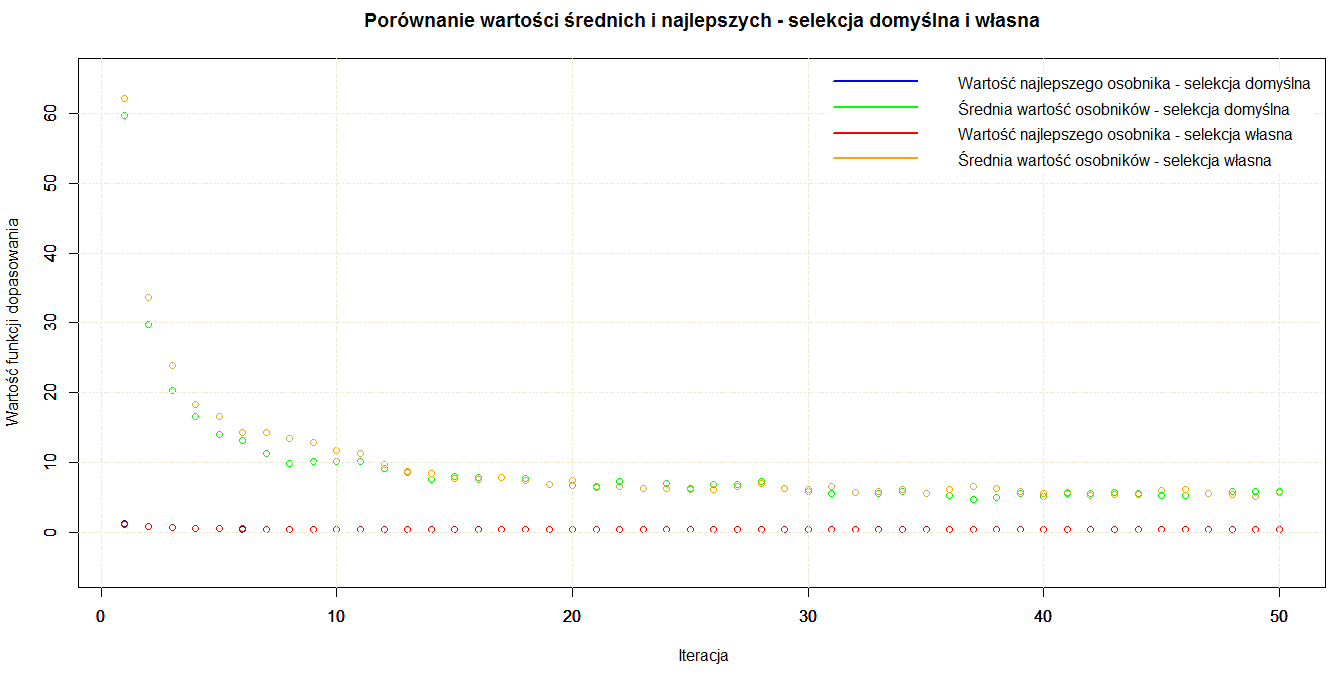
\includegraphics[scale = 0.5]{img/zad1/sel_20}
	\caption{Wykres przy 20 osobnikach elitarnych}  
	\label{rys:sel_20} 
\end{figure}

\begin{figure}[H]
	\centering
	\hspace*{-0.8in}
	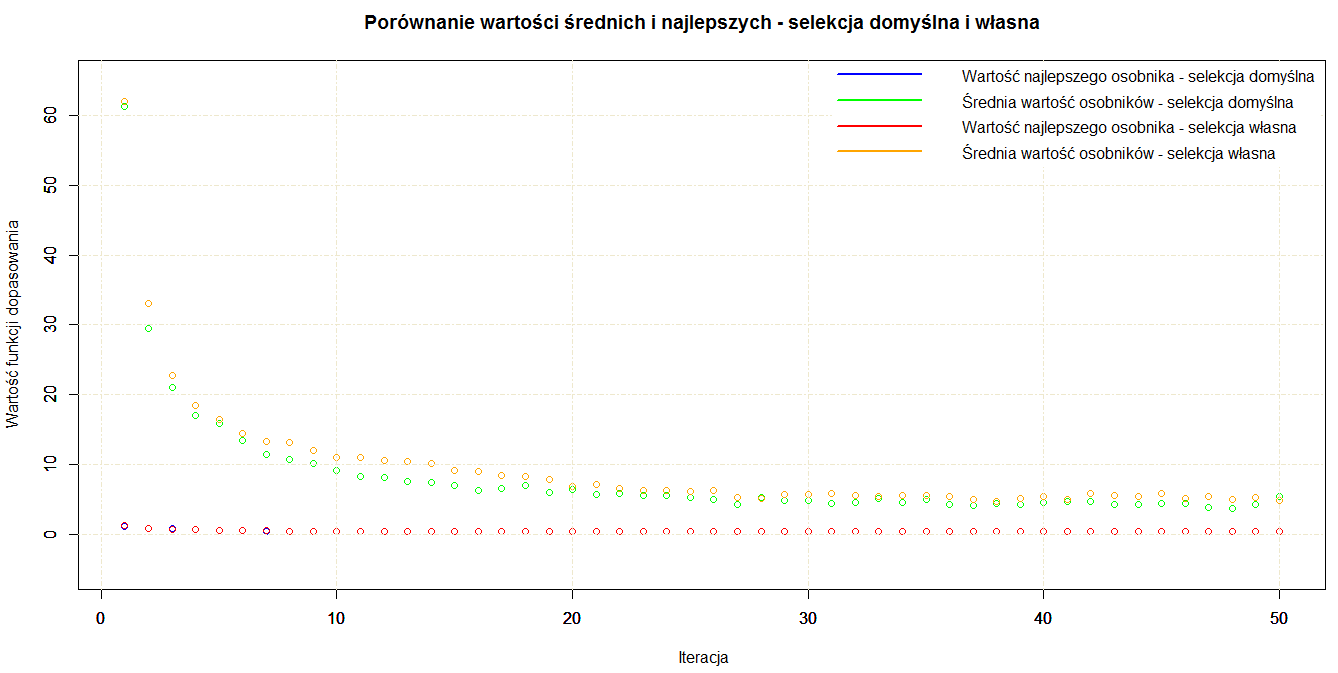
\includegraphics[scale = 0.5]{img/zad1/sel_50}
	\caption{Wykres przy 50 osobnikach elitarnych}  
	\label{rys:sel_50} 
\end{figure}

\subsubsection{Wnioski}

\begin{table}[!h]
	\centering
	\caption{Wartości średnie i najlepsze osobnika dla domyślnej i własnej funkcji selekcji}
	\label{sel_porownanie}
	\begin{tabular}{|c|c|c|c|c|}
		\hline
		\textbf{Selekcja} & \multicolumn{2}{c}{\textbf{Selekcja domyślna}}  & \multicolumn{2}{|c|}{\textbf{Selekcja własna}} \\ \cline{2-5}
		\textbf{elitarna} & Wartość średnia & Najlepszy wynik & Wartość średnia & Najlepszy wynik \\ \hline
		
		1  & 13.660880  & 0.405495 & 22.860800 & 0.414707 \\
		6  & 7.106856 & 0.400895 & 5.544652 & 0.397909 \\
		20 & 5.847374 & \textbf{{\color{green} 0.397888 }} & 5.678752 & 0.397977 \\
		50 & 5.42606 & 0.397903 & 4.833812 & \textbf{{\color{green} 0.397888 }} \\ \hline      
	\end{tabular}
\end{table}

Najlepsze wyniki zarówno dla selekcji domyślnej, jak i własnej, pojawiają się przy większych ilościach osobników elitarnych (różnią się o 1 na szóstej pozycji po przecinku od minimum globalnego). Można zauważyć, że nowa funkcja selekcji działa nieco inaczej i najlepsze rezultaty daje przy liczbie osobników elitarnych równej aż połowie populacji.\\
Natomiast dla 1 osobnika elitarnego przy użyciu zaimplementowanej funkcji wartości średnie osobników znaczie odstają od tych uzyskanych za pomocą selekcji pochodzącej z pakietu \textit{GA}, także najlepsze wyniki nie są zbliżone do minimum lokalnego.